\documentclass[10pt,conference,compsocconf]{IEEEtran}

\usepackage{xltxtra}
\usepackage{tabularx}
\usepackage{booktabs}
\usepackage[caption=false]{subfig}
\usepackage[numbers,sort&compress]{natbib}
%\setmainfont{Times New Roman}

\begin{document}

\title{idock: A Multithreaded Virtual Screening Tool for Flexible Ligand Docking}

\author{\IEEEauthorblockN {Hongjian Li\IEEEauthorrefmark{1}, Kwong-Sak Leung\IEEEauthorrefmark{1} and Man-Hon Wong\IEEEauthorrefmark{1}
\IEEEauthorblockA {\IEEEauthorrefmark{1} Department of Computer Science and Engineering\\
Chinese University of Hong Kong\\
Shatin, New Territories, Hong Kong, P.R. China\\
Email: hjli@cse.cuhk.edu.hk}}}

\maketitle

\begin{figure*}
\centering
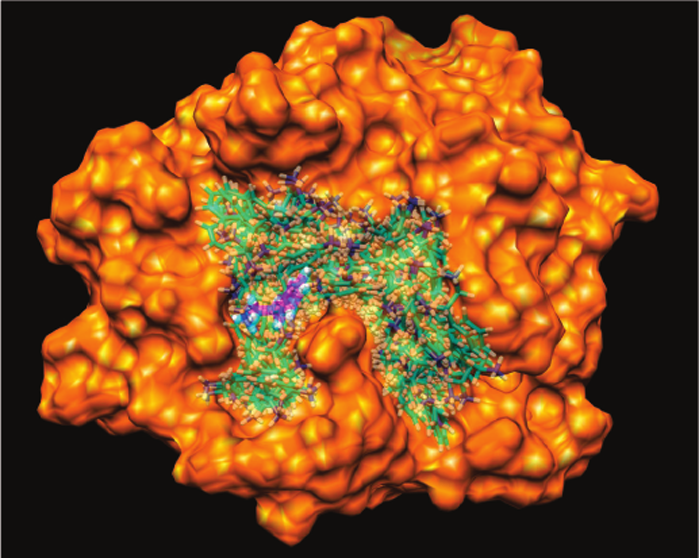
\includegraphics[width=\linewidth]{Figures/Decoys.png}
\caption{Flexible-ligand binding decoys.}
\label{fig:decoys}
\end{figure*}

\begin{table*}
\centering
\begin{tabular*}
{\linewidth}
{@{\extracolsep{\fill}}rrrr}
\toprule
& Total records & No. of native ligands & No. of decoys\\
\midrule
\multicolumn{4}{l}{\textbf{Raw csv files}}\\
set 1 & 138,621 & 176 & 138,445\\
set 2 & 130,791 & 167 & 130,624\\
\noalign{\smallskip\smallskip}
\multicolumn{4}{l}{\textbf{Case study 1}}\\
set 1 & 347 & 176 & 171\\
set 2 & 331 & 167 & 164\\
\noalign{\smallskip\smallskip}
\multicolumn{4}{l}{\textbf{Case study 2}}\\
set 1 & 3,473 & 1,760 & 1,713\\
set 2 & 3,310 & 1,670 & 1,640\\
\noalign{\smallskip\smallskip}
\multicolumn{4}{l}{\textbf{Case study 3}}\\
set 1 & 276,890 & 138,445 & 138,445\\
set 2 & 261,248 & 130,624 & 130,624\\
\bottomrule
\end{tabular*}
\caption{Number of native ligand conformations and decoys in set 1 and set 2 in raw csv files and case studies 1, 2 and 3.}
\label{tab:sets_stats}
\end{table*}

\begin{figure*}
\centering
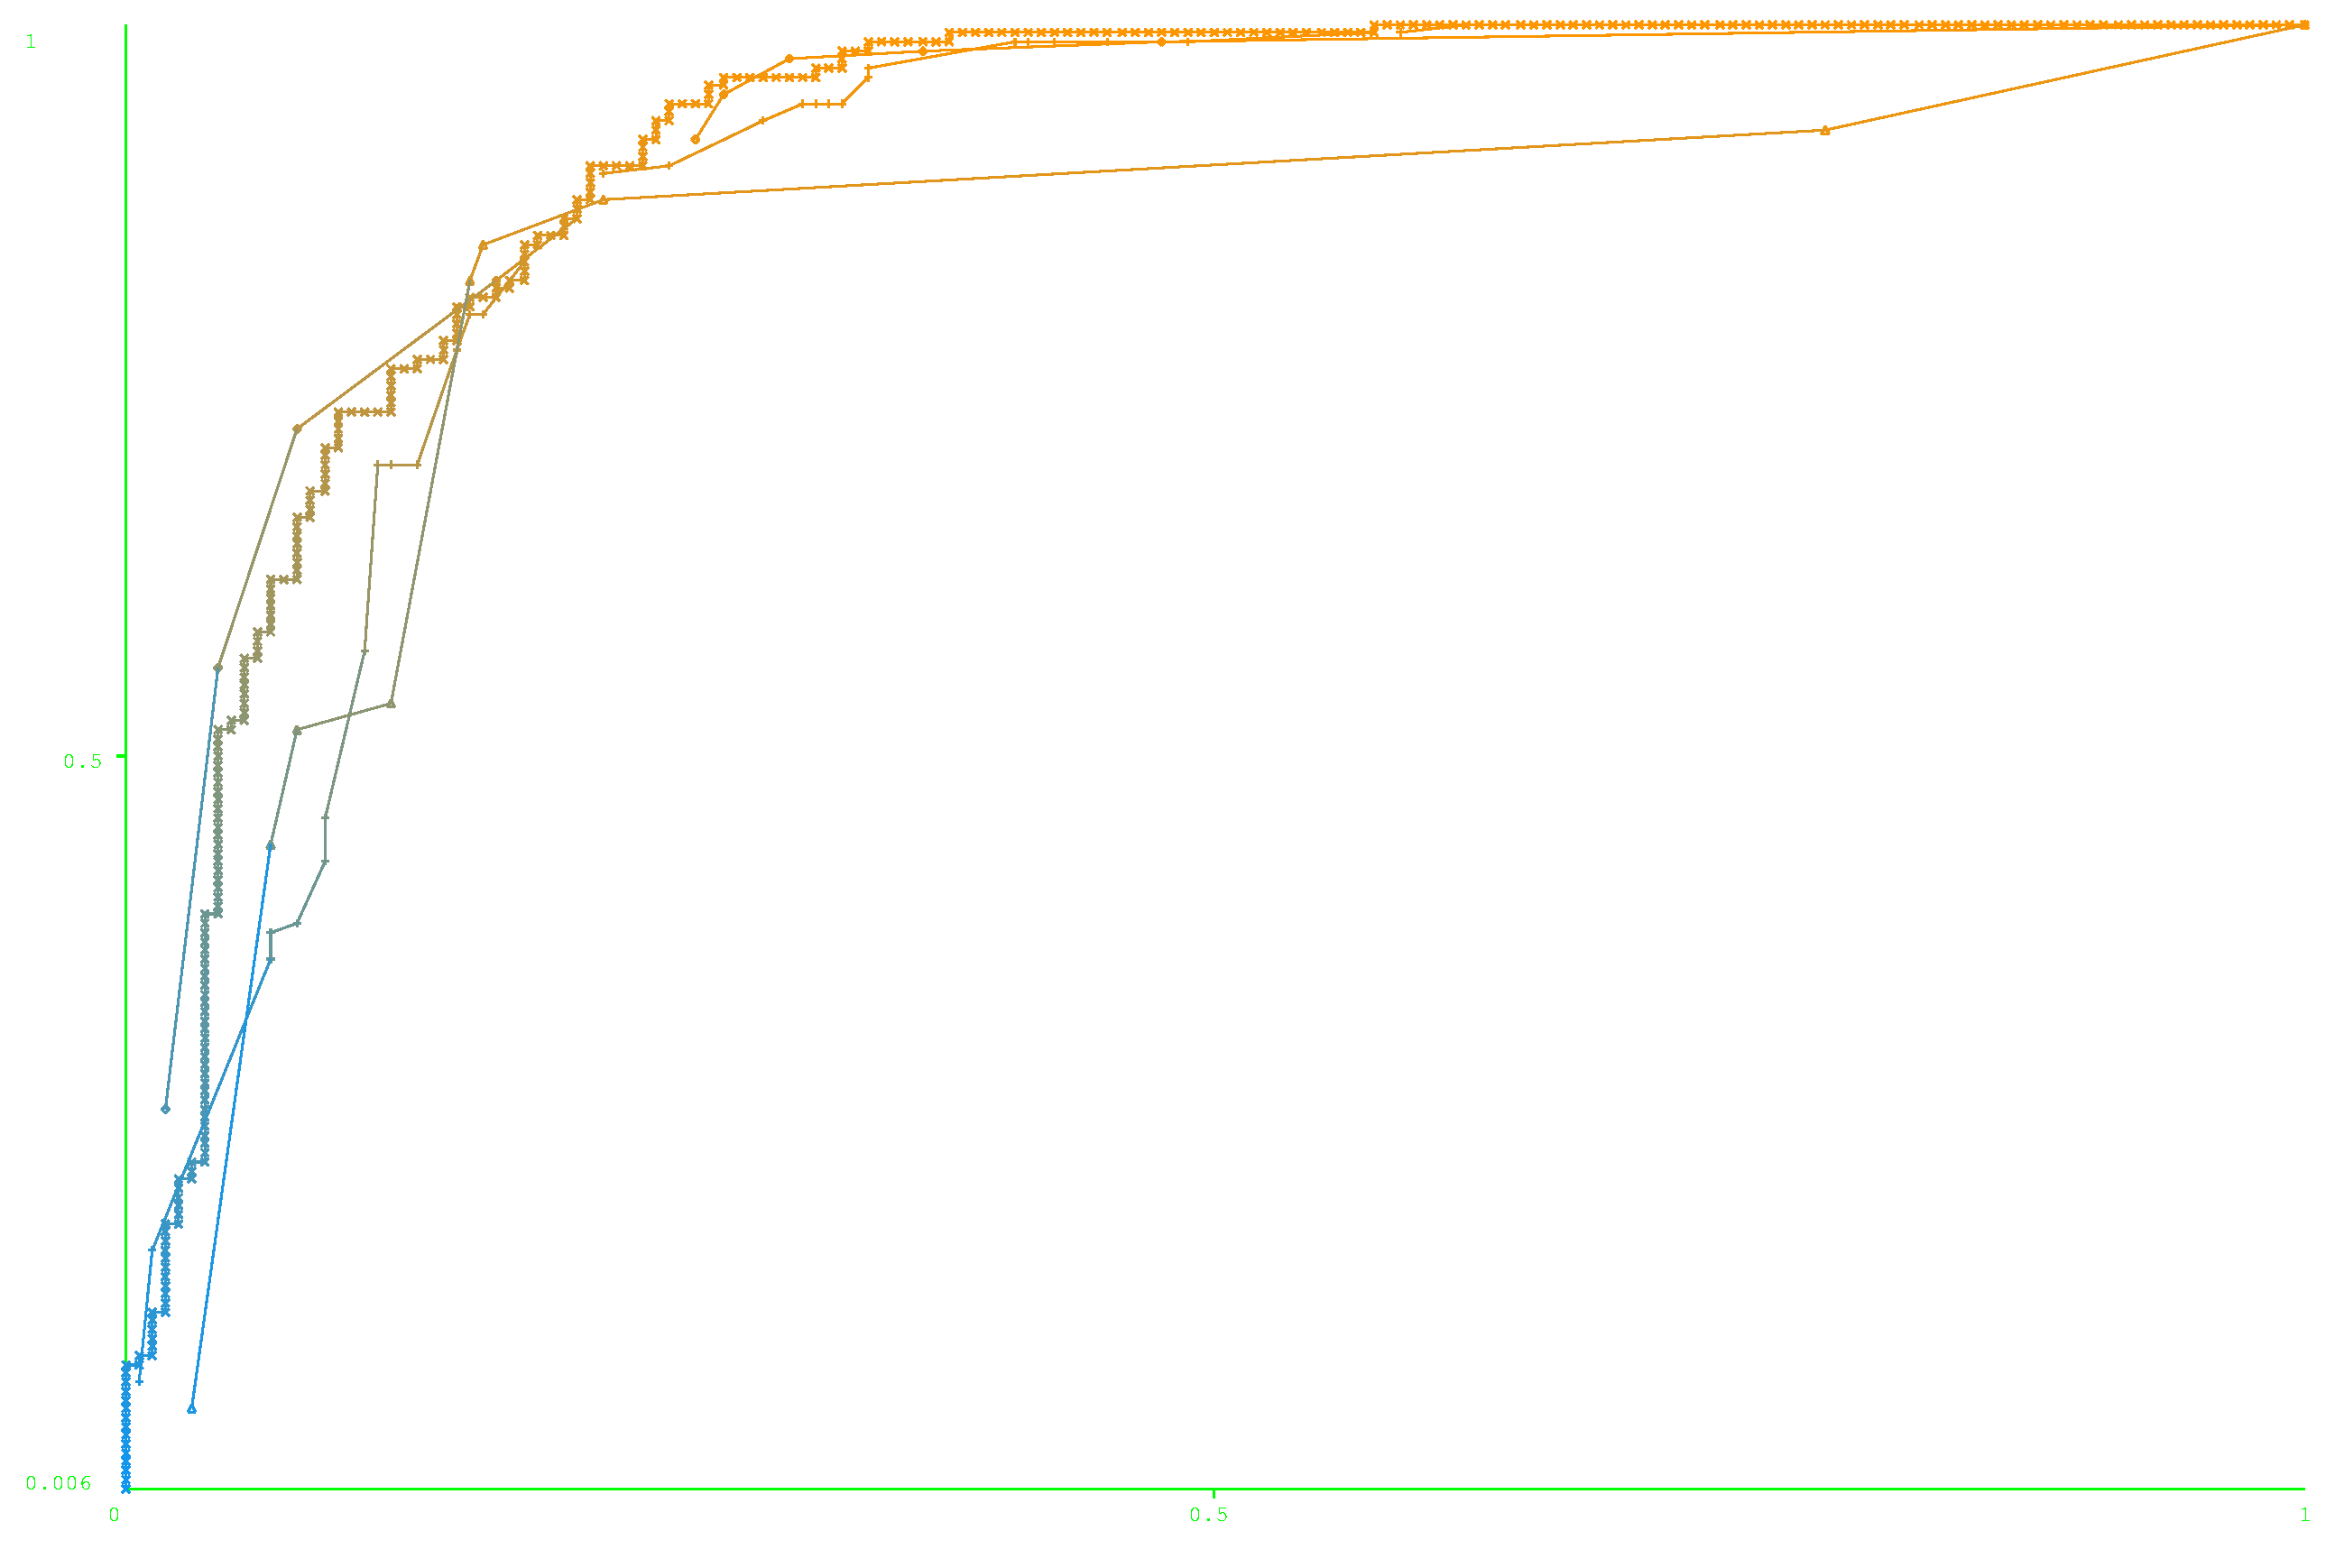
\includegraphics[width=\linewidth]{Figures/l1_f50/t1T2/roc.eps}
\caption{set1.}
\label{fig:set1}
\end{figure*}

\begin{figure}
\centering
\begin{tabular}{cc}
\subfloat[active.]
{
  \label{subfig:l1_f50_set1_active}
  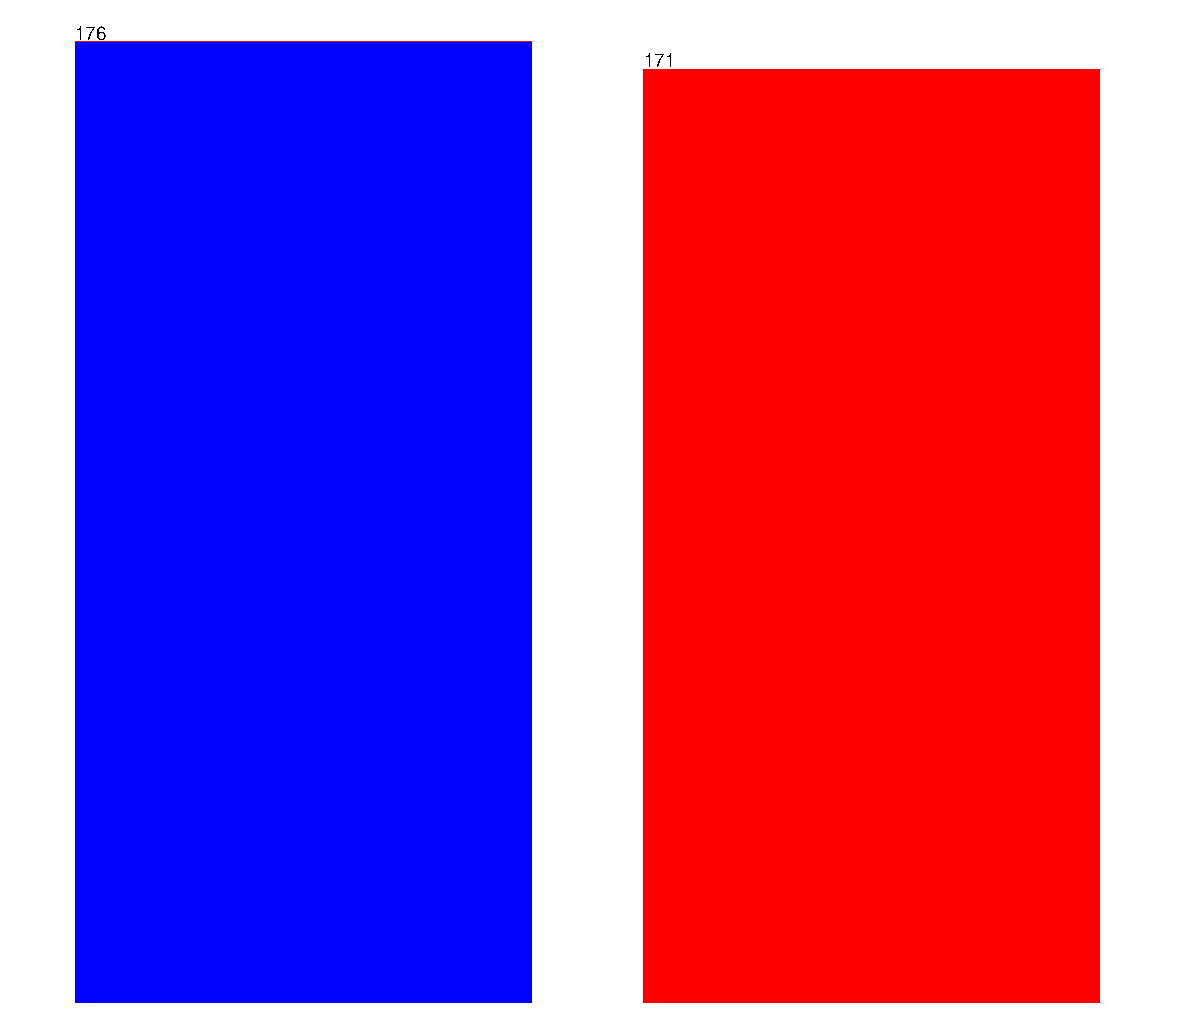
\includegraphics[width=0.46\linewidth]{Figures/l1_f50/set1/active.eps}
} &
\subfloat[gauss 1.]
{
  \label{subfig:l1_f50_set1_gauss1}
  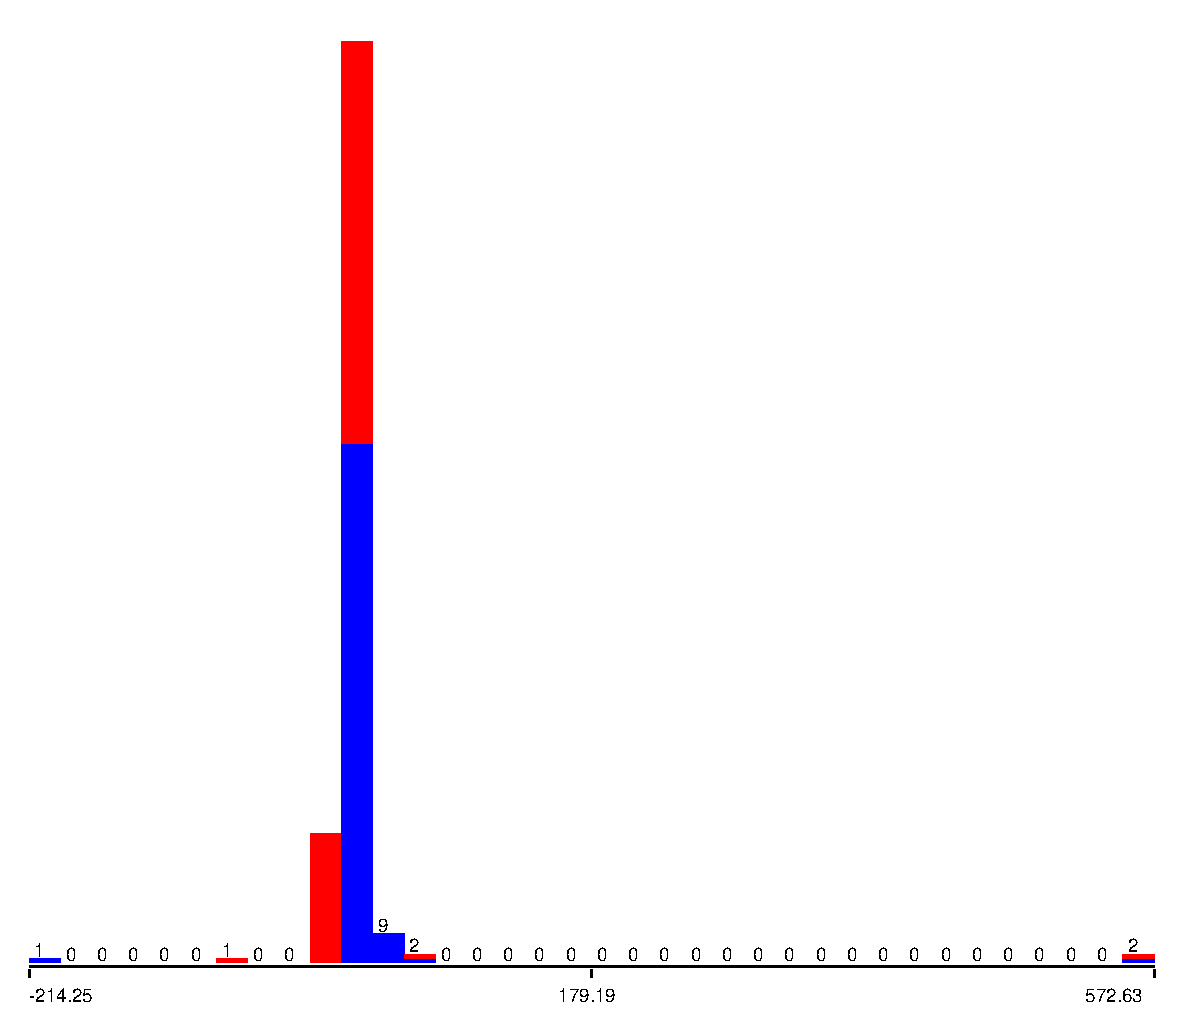
\includegraphics[width=0.46\linewidth]{Figures/l1_f50/set1/gauss1.eps}
} \\
\subfloat[gauss 2.]
{
  \label{subfig:l1_f50_set1_gauss2}
  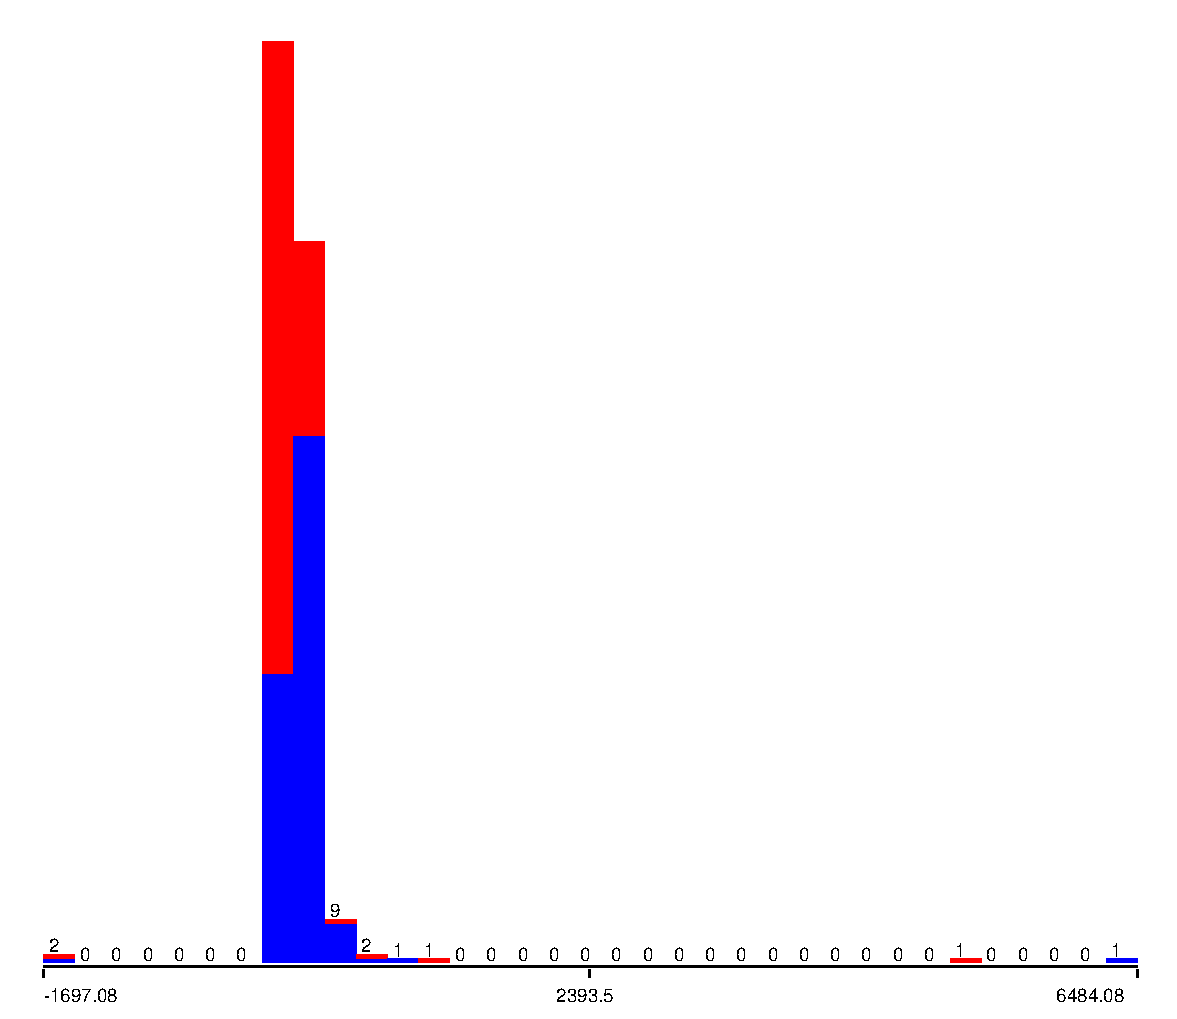
\includegraphics[width=0.46\linewidth]{Figures/l1_f50/set1/gauss2.eps}
} &
\subfloat[repulsion.]
{
  \label{subfig:l1_f50_set1_repulsion}
  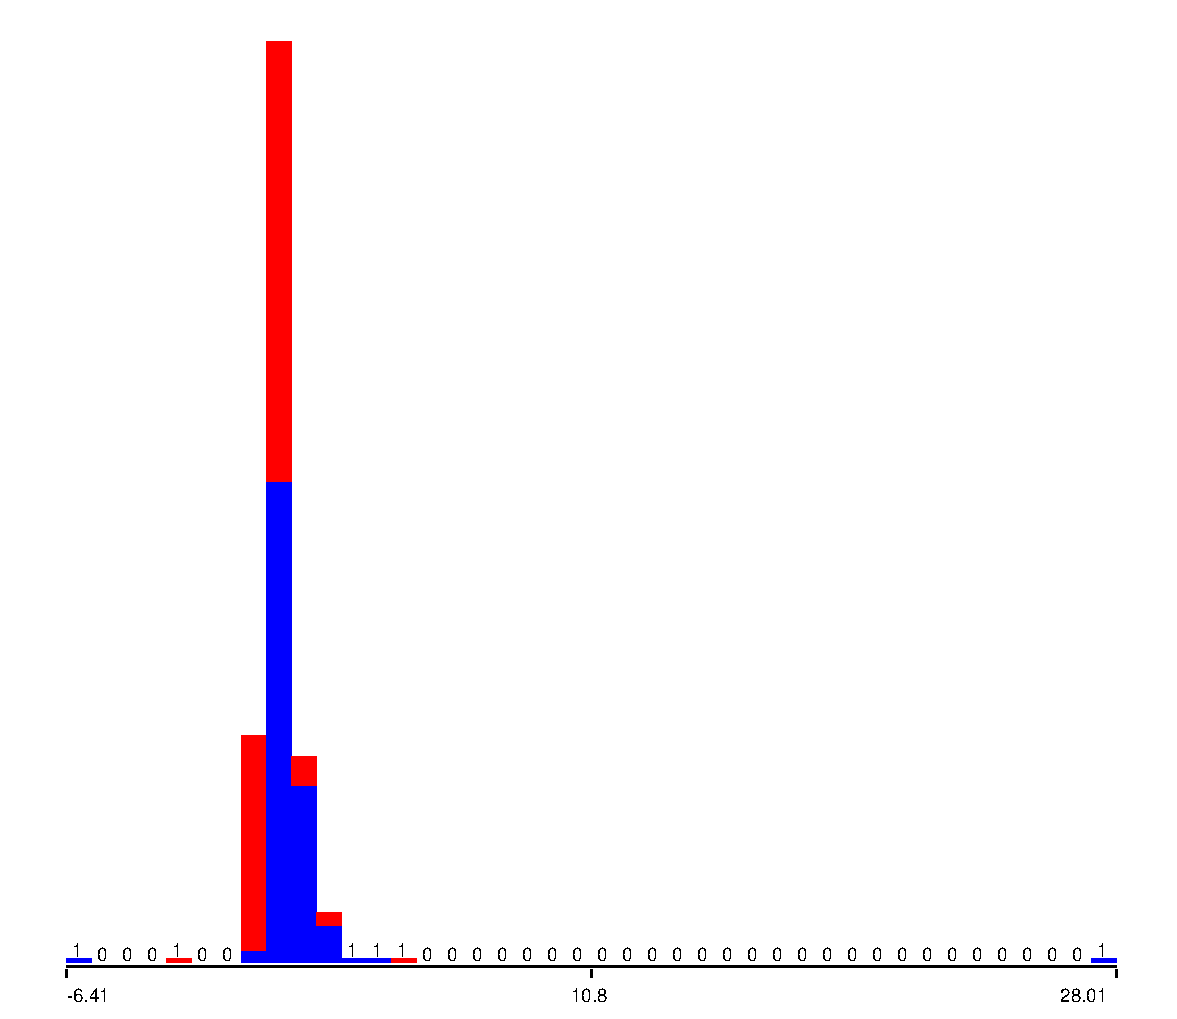
\includegraphics[width=0.46\linewidth]{Figures/l1_f50/set1/repulsion.eps}
} \\
\subfloat[hydrophobic interaction.]
{
  \label{subfig:l1_f50_set1_hydrophobic}
  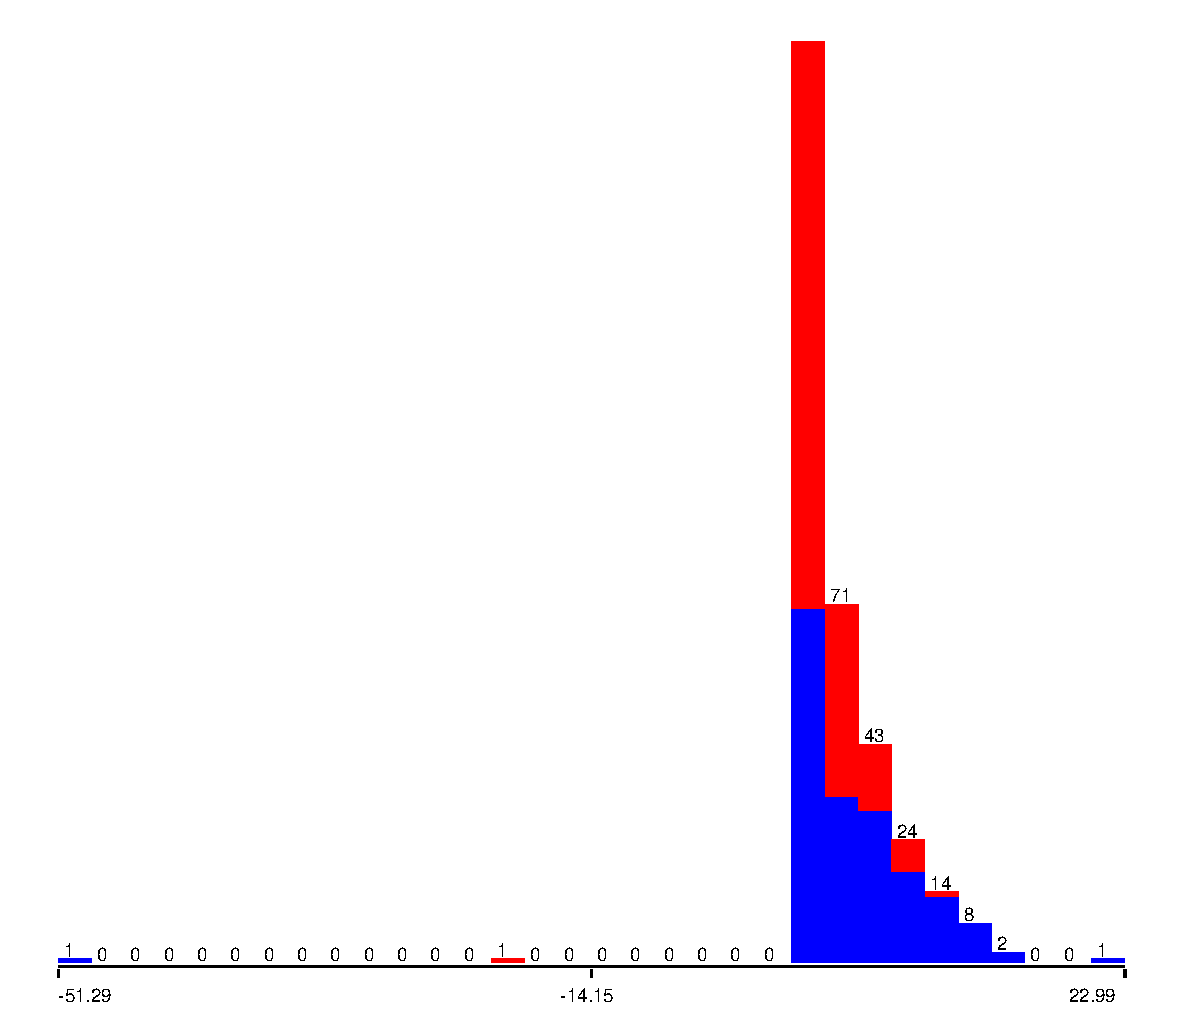
\includegraphics[width=0.46\linewidth]{Figures/l1_f50/set1/hydrophobic.eps}
} &
\subfloat[hydrogen bonding.]
{
  \label{subfig:l1_f50_set1_hydrogenbonding}
  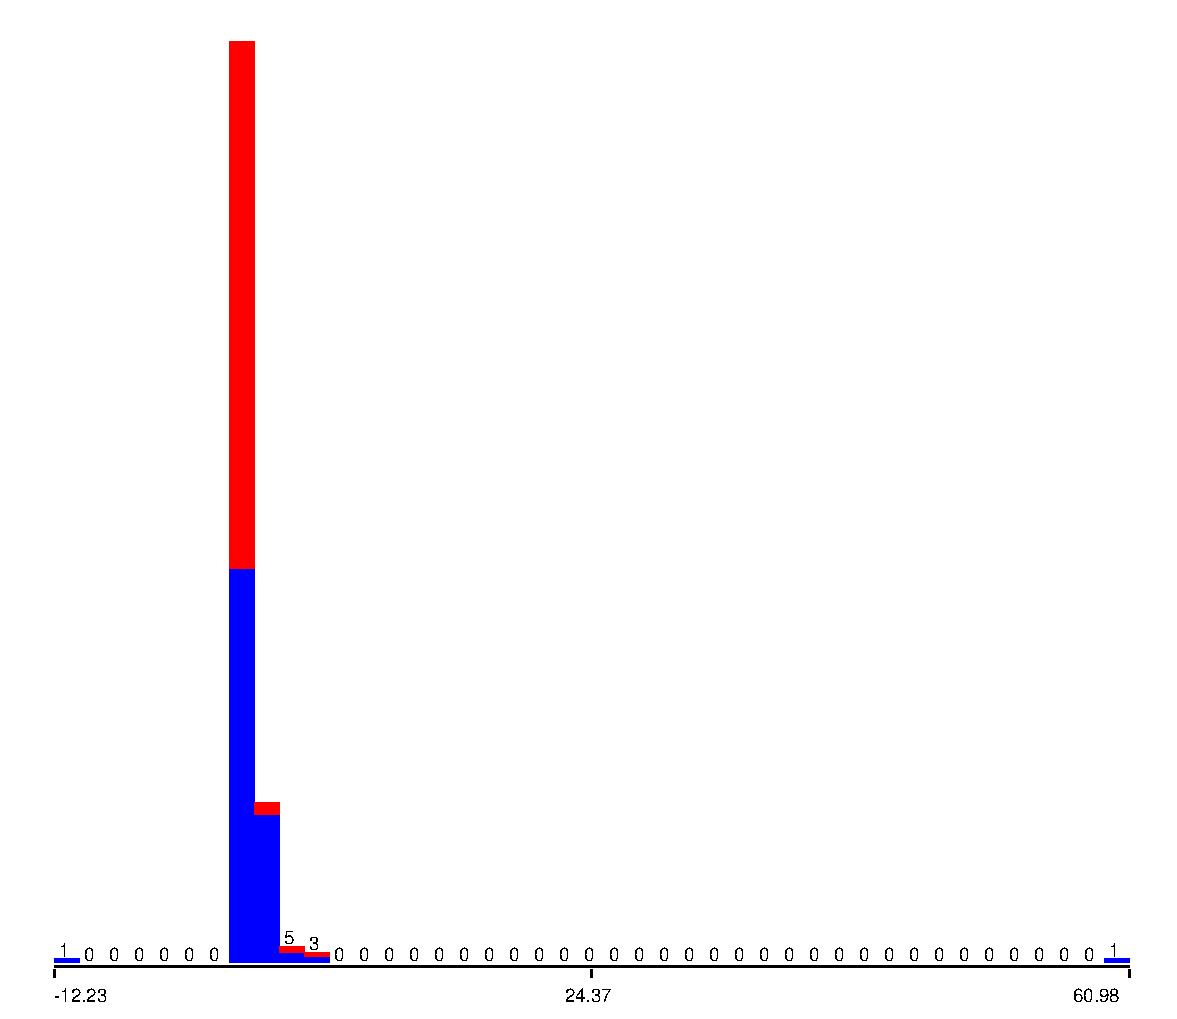
\includegraphics[width=0.46\linewidth]{Figures/l1_f50/set1/hydrogenbonding.eps}
} \\
\end{tabular}
\caption{Distributions of the 5 feature attributes and the binary class attribute of set 1 in case study 1. Class 1 is rendered in blue and class 0 is render in red.}
\label{fig:l1_f50_set1_dists}
\end{figure}



In \citeyear{970}, \Citeauthor{970} developed a program.

B \citep{698} and C \citep{299} and D \citep{777}.

\citep{967,968,969}

\bibliographystyle{unsrtnat}
\bibliography{../refworks}

\end{document}

